\chapter{Komunikacja w układzie}

Przesyłanie danych pomiędzy czujnikami a stacją główną (mikrokomputerem) jest najistotniejszą częścią całego układu. System pomiarów, po poprawnym, sprzętowym podłączeniu każdego z podzespołów, należy następnie skomunikować. Urządzenia pomiarowe wraz z głównym komputerem można komunikować poprzez interfejsy cyfrowe zaimplementowane w danym urządzeniu. Mikrokomputer BeagleBone Black obsługuje kilka interfejsów komunikacji: SPI, $\mathbf{I^{2}C}$, 1-Wire, CAN, UART. Możliwa jest również łączność poprzez zwykłe porty GPIO (General Purpose Input/Output).

\section{Magistrala szeregowa $\mathbf{I^{2}C}$}
Magistrala jest to układ linii, po których przekazywane są wszystkie informacje pomiędzy podłączonymi do niej urządzeniami, np. komputerem, czujnikiem, regulatorem itp. Zasada działania magistrali opiera się na uzyskiwaniu oraz nadawaniu współpracującym częściom uprawnień do transmisji danych w danej jednostce czasu. W jednej chwili, w magistrali może działać tylko jedno urządzenie nadające oraz dowolna liczba odbiorców. Systemy o budowie opartej na magistrali są łatwo modyfikowalne oraz rozszerzalne, w prosty sposób można dołączyć lub odłączyć elementy systemu.
Dane przesyłane na dużą odległość najlepiej jest przekazywać transmisją szeregową, na krótsze odległości, przesyłanie równoległe oraz szeregowe daje podobne rezultaty.
Bity oraz całe słowa w tej komunikacji przesyłane są jeden po drugim. Przy takim sposobie łączenia się wystarczą tylko dwa przewody łączące odbiorcę z urządzeniem nadającym. 

Przykład urządzenia w magistrali szeregowej został przedstawiony na  rysunku \ref{fig:magistrala}.
\begin{figure}[h]
\centering
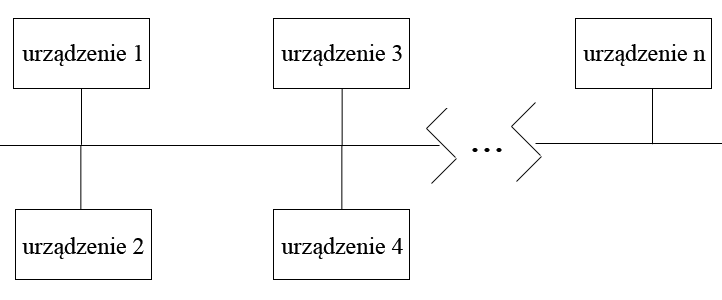
\includegraphics[scale=0.5]{magistrala}
\caption{Schemat magistrali szeregowej}
\label{fig:magistrala}
\end{figure}

Jak widać na załączonym schemacie, można podłączyć do magistrali wiele urządzeń. Wszystkie są podłączone do jednej lini danych, na której odbywa się komunikacja. To właśnie przez nią przesyłane są wszystkie dane pomiędzy elementami magistrali.


Nazwa magistrala szeregowej $\mathbf{I^{2}C}$ jest akronimem od Inter-Intergrated Circuit. Standard został opracowany w latach osiemdziesiątych przez firmę Philips.

Jest ona bardzo często wykorzystywana w układach mikroprocesorowych, w sterownikach wyświetlaczy LCD, można ją stosować do sterowania pamięci RAM, EPROM, układami I/O.

Zaletami magistrali $I^{2}C$ są niewątpliwie takie właściwośći jak: odporność na zakłócenia zewnętrzne, dodtakowe układu podłączone do niej mogą być dodawane lub wyłączone bez ingerencji w pozostały układ połączeń wcześniej stworzonych, połączenie na magistrali składają się tylko z dwóch przewodów, przez co ich ogólna liczba jest minimalizowana, wykrywanie błędów jest proste i łatwe do analizy, na magistrali może znajdować się wiele urządzeń typu master, umożliwiając kontrolę gotowych układów przez zewnętrzny komputer.

Magistrala $I^{2}C$ posiada dwie dwukierunkowe linie: dane są przesyłane przez Serial Data (SDA), natomiast sygnał zegara na Serial Clock (SCL).
